
\section{Nucleosynthesis}
\label{ohno:sec:yields}

% fig 2
\begin{figure*}
\centering
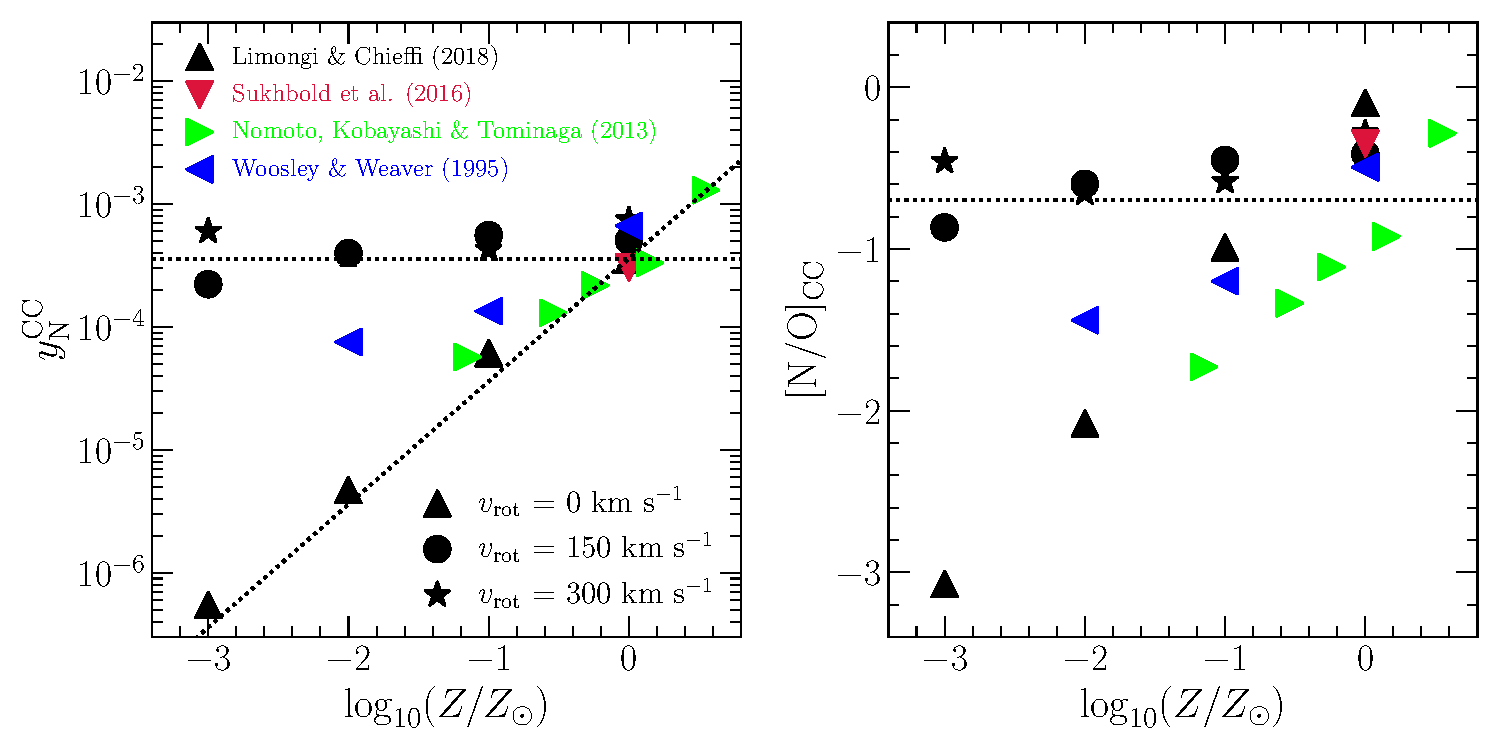
\includegraphics[scale = 0.65]{n_cc_yields.pdf}
\caption{
\textbf{Left}: IMF-averaged CCSN yields of N calculated using~\vice's
\texttt{vice.yields.ccsne.fractional} function with the tables published by
\citet[][blue]{Woosley1995},~\citet[][green]{Nomoto2013},
\citet[][red]{Sukhbold2016}, and~\citet[][black]{Limongi2018}.
All studies report yields for non-rotating progenitors, shown by the triangles;
for visual clarity, the triangles point in a different direction for each study
according to the legend.
\citet{Limongi2018} report additional yields for progenitors with rotational
velocities of 150 (circles) and 300 km/s (stars).
The horizontal dashed line marks~$\ycc{N} = 3.6\times10^{-4}$,
the value of our fiducial CCSN yield of N in our GCE models.
We also use the form shown by the slanted line (equation~\ref{ohno:eq:linear_yncc})
in~\S~\ref{ohno:sec:results:yields:yncc} in combination with some of our AGB star
yield models discussed in~\S~\ref{ohno:sec:yields:agb}.
\textbf{Right}: The~\no~ratio predicted by each of the explosion models in
the left-hand panel, under the same colour-coding and marker scheme.
We mark the position of~$\no = -0.7$ with a black dotted line, the value
roughly suggested by the observations of low-metallicity systems highlighted
in Fig.~\ref{ohno:fig:no_oh_observed}.
}
\label{ohno:fig:n_cc_yields}
\end{figure*}

Here we make use of the chemical evolution model for the Milky Way
presented by~\citet{Johnson2021}, which runs using the publicly available
\texttt{Versatile Integrator for Chemical Evolution}
(\vice, see Appendix~\ref{ohno:sec:vice};~\citealp{Johnson2020, Griffith2021b,
Johnson2021}), an open-source~\python~package designed for GCE modeling.
\citet{Johnson2021} focus their discussion of the model predictions on O and
Fe, and we retain their yields of these elements here.
The supernova (SN) yields are defined as the net mass of some element X
produced over all explosion events in units of the progenitor cluster's mass.
For example, with a yield of~$y_\text{X} = 0.001$, a hypothetical~$1000~\msun$
star cluster would produce~$1~\msun$ of the element X instantaneously in the
case of core-collapse supernovae (CCSNe) or over the delay-time distribution
(DTD) in the case of SNe Ia.
These yields are net yields in that they do not include the metal mass
ejected to the ISM that was initially present within a star; in the previous
example, the~$1~\msun$ yield is only the newly produced metal mass.
% {\color{red}
In GCE models,~\vice~implements an additional return of
previously produced nucleosynthetic material from stellar envelopes at their
birth composition (for details, see discussion in~\citealt{Johnson2020},
\citealt{Johnson2021}, and the~\vice~science documentation).
% }
We adopt the following values from~\citet{Johnson2021}:
\begin{itemize}
	\item $\ycc{O} = 0.015$

	\item $\ycc{Fe} = 0.0012$

	\item $\yia{O} = 0$

	\item $\yia{Fe} = 0.00214$,
\end{itemize}
where the subscripts and superscripts differentiate between the element and the
SN type.
\par
These choices are based on a mix of theoretical and empirical considerations.
For a~\citet{Kroupa2001} IMF,
% {\color{red} \sout{initial mass function (IMF)} IMF},
the solar metallicity CCSN yields of~\citet{Chieffi2013}
and~\citeauthor{Griffith2021b} (\citeyear{Griffith2021b}, based on
the~\citealt{Sukhbold2016} models with forced explosions).
predict~$\ycc{O} = 0.016$ and 0.018, respectively, if all stars
from~$8 - 120~\msun$ explode.
The value of~$\ycc{O} = 0.015$ allows for a modest amount of black hole
formation but implicitly assumes that most massive stars explode.\footnote{
	If all stars from~$8 - 40~\msun$ explode and all more massive stars
	collapse, then the~\citet{Sukhbold2016} models with forced explosions
	yield~$\ycc{O} = 0.013$~\citep{Griffith2021b}.
}
% {\color{red}
% \sout{In chemical evolution models, this choice of yield also leads to good
% agreement with the observationally inferred deuterium-to-hydrogen ratio of the
% local ISM~\mbox{\citep{Linsky2006}}, while substantially lower~$\ycc{O}$ leads
% to disagreement~\mbox{\citep{Weinberg2017b}}.}
While ratios of effective yields can be reasonably constrained with observed
abundance ratios~\citep[e.g.,][]{Weinberg2019, Weinberg2022, Griffith2021b,
Griffith2022}, their absolute scale is strongly degenerate with the strength of
mass-loading in Galactic winds.
In GCE models, our choice of normalization leads to good agreement with the
observationally inferred deuterium-to-hydrogen ratio of the local ISM
\citep{Linsky2006}, while substantially lower~$\ycc{O}$ leads to disagreement
\citep{Weinberg2017b}.
However, there are a number of models that reproduce observed abundance
patterns of other elements in the Milky Way with weak or negligible outflows
and a much lower yield normalization (e.g.,~\citealp*{Kubryk2015b};
\citealp{Prantzos2018, Spitoni2019, Spitoni2021}).
We explore variations of the absolute scale of nucleosynthetic yields and
outflows in~\S~\ref{ohno:sec:results:yields:variations} below and find that our
conclusions are not impacted by the assumed normalization.
% }
\par
Our adopted values of~\ycc{O}~and~\ycc{Fe}~give~$\ofe\approx0.43$ for stars
with pure CCSN enrichment, in good agreement with the ``high-$\alpha$'' plateau
of disk stars found by~\citet{Ramirez2013}; matching the APOGEE plateau
at~$\ofe\approx0.35$~\citep[see, e.g., fig.~6 of][]{Hasselquist2021} would
instead require a slightly higher~$\ycc{Fe} = 0.0014$.
SN Ia models predict minimal O yields, justifying~$\yia{O} = 0$.
The choice of~$\yia{Fe} = 0.00214$ then leads to good agreement with the
observed~\ofe~values of low-$\alpha$ thin-disc stars given the star formation
assumptions used by~\citeauthor{Johnson2021} (\citeyear{Johnson2021}; for
analytic discussion, see~\S~3.1 of~\citealp{Weinberg2017b}).
For an Fe yield of~$0.77~\msun$ from a single SN Ia event~\citep{Iwamoto1999},
this~\yia{Fe}~corresponds to a time-integrated SN Ia rate
of~$R_\text{Ia} = 2.7\times10^{-3}~\msun^{-1}$ (i.e., 2.7 SNe Ia per
1000~\msun~of star formation), which is moderately higher than the value
of~$2.2\times10^{-3}~\msun^{-1}$ inferred by~\citet{Maoz2012a} for
a~\citet{Kroupa2001} IMF.
Our choice of yields is internally consistent and reproduces many Milky Way
observations~\citep{Johnson2021}, but many of the GCE model predictions would
be minimally affected if we lowered~\ycc{O},~\ycc{Fe}, and~\yia{Fe}~by a
common factor and reduced the efficiency of outflows.
We return to this point in the context of N yields
in~\S~\ref{ohno:sec:results:yields:variations}.
\par
We assume that N is not produced in significant amounts by SNe Ia
\citep{Johnson2019}, setting~$\yia{N} = 0$.
The remainder of this section discusses the CCSN and AGB star yields of N.
\par
A significant portion of N yields arise as a consequence of the CNO
cycle.
% \footnote{
% 	\color{red}
% 	\sout{
% 	\Ctwelve(p,~$\gamma$)\Nthirteen($\beta^+~\nu_\text{e}$)\Cthirteen
% 	(p,~$\gamma$)\Nfourteen(p,~$\gamma$)\Ofifteen($\beta^+~\nu_\text{e}$)
% 	\Nfifteen(p,~$\alpha$)\Ctwelve
% 	}
% }
As the dominant source of pressure and energy generation in non-zero
metallicity main sequence stars with initial masses of~$\gtrsim$1.3~\msun, this
cyclic nuclear reaction catalyses the conversion of H into He that would
otherwise be accomplished by the proton-proton chain
(\citealp{vonWeizsaecker1937, vonWeizsaecker1938, Bethe1939a, Bethe1939b,
Adelberger2011};~\citealp*{Suliga2021}).
Its slowest component by far is the~\Nfourteen(p,~$\gamma$)\Ofifteen~reaction
\citep[e.g.][]{LUNACollaboration2006}.
Consequently, the first order effect of the CNO cycle is to convert most of the
C isotopes in stellar cores into~\Nfourteen.
As we will discuss in this section, this plays an important role in shaping N
yields from stars of all masses.

\subsection{Core Collapse Supernovae and Massive Star Winds}
\label{ohno:sec:yields:ccsne}

In~\vice, CCSN nucleosynthetic products are approximated to be produced
instantaneously following an episode of star formation; this is a good
approximation because the lives of massive stars are short compared to the
relevant timescales for GCE.
The yield is simply the constant of proportionality between the CCSN production
rate and the star formation rate (SFR):
\begin{equation}
\dot{M}_\text{X}^\text{CC} = \ycc{X}\dot{M}_\star
\end{equation}
More generally,~\ycc{X}~quantifies~\textit{all} of the nucleosynthetic material
approximated to be produced instantaneously following a single stellar
population's formation, including newly synthesized material expelled in a
massive star wind before the star explodes or collapses to a black hole.
\par
We compute theoretically predicted values of~\ycc{N}~using
\vice's~\texttt{vice.yields.ccsne.fractional} function assuming a
\citet{Kroupa2001} IMF; details on how~\vice~handles these calculations can be
found in~\S~4 of~\citet{Griffith2021b} and in the~\vice~science 
documentation\footnote{\url
	{https://vice-astro.readthedocs.io/en/latest/science_documentation/yields}
}.
In the left panel of Fig.~\ref{ohno:fig:n_cc_yields}, we plot the results as a
function of progenitor metallicity as predicted by the~\citet{Woosley1995},
\citet*{Nomoto2013},~\citet{Sukhbold2016}, and~\citet{Limongi2018} tables.
There is generally good agreement between the various non-rotating models, but
only~\citet{Limongi2018} report yields for progenitors with non-zero rotational
velocities; these yields are substantially larger than their non-rotating
counterparts, especially at low metallicity.
With few seed nuclei for the CNO cycle at low~$Z$, production of~\Nfourteen~is
difficult.
Rotation-induced mixing, a highly uncertain process~\citep{Zahn1992, Maeder1998,
Lagarde2012}, could transport newly produced C and O into the hydrogen burning
shell of the CCSN progenitor, facilitating~\Nfourteen~production
(\citealp{Frischknecht2016}; see also discussion in~\S~4.2 of
\citealp{Andrews2017}).
Consequently, N yields at low metallicity are quite sensitive to model-dependent
assumptions regarding stellar rotation and internal mixing processes
\citep{Heger2010}.
\par
We compute the~\no~ratio of CCSN ejecta from the values
of~\ycc{N}~and~\ycc{O}~predicted by a given yield table according to
\begin{equation}
\no\subcc = 
\log_{10}\left(\frac{\ycc{N}}{\ycc{O}}\right) -
\log_{10}\left(\frac{Z_{\text{N},\odot}}{Z_{\text{O},\odot}}\right),
\label{ohno:eq:no_subcc}
\end{equation}
where~$Z_{\text{X},\odot}$ is the abundance by mass of some element X in the
sun, for which we take~$Z_{\text{N},\odot} = 6.91\times10^{-4}$ and
$Z_{\text{O},\odot} = 5.72\times10^{-3}$ based on the photospheric measurements
of~\citet{Asplund2009}.
For each value of~\ycc{N}~in the left panel of Fig.~\ref{ohno:fig:n_cc_yields}, we
compute the corresponding values of~\ycc{O}~and illustrate the
resultant~\no\subcc~ratios in the right panel.
These yield ratios follow similar trends with progenitor metallicity and
rotation as~\ycc{N}~itself, a consequence of the fact that these
studies predict relatively metallicity- and rotation-independent O yields.
At low metallicity, CCSN yields of N dominate over the AGB star yields (see
discussion in~\S~\ref{ohno:sec:yields:agb}), and Fig.~\ref{ohno:fig:no_oh_observed}
suggests a plateau in~\no~at low metallicity at~$\no\subcc\approx-0.7$.
% {\color{red}
We have examined versions of Fig.~\ref{ohno:fig:n_cc_yields} with shallow and steep
variations of the~\citet{Kroupa2001} IMF (i.e., power-law indices
$\gamma = -2.0$ and~$-2.6$, respectively).
This level of IMF variability produces factor of~$\sim$$2$ variations in
$\ycc{N}$, but the~\no\subcc~ratios are nearly unaffected because massive star
yields of N and O follow similar trends with stellar mass.
% }
Taking this value in combination with our adopted O yield of~$\ycc{O} = 0.015$,
equation~\refp{ohno:eq:no_subcc} suggests that~$\ycc{N} = 3.6\times10^{-4}$.
We highlight both~\no\subcc~=~$-0.7$ and~$\ycc{N} = 3.6\times10^{-4}$ with
horizontal black dashed lines in Fig.~\ref{ohno:fig:n_cc_yields}, finding good
agreement with the rotating progenitor models of~\citet{Limongi2018} in both
panels.
This indicates that rotating massive stars play an important role in
establishing the N abundances at low metallicity, in agreement with previous
works~\citep{Chiappini2003, Chiappini2005, Chiappini2006, Kobayashi2011,
Prantzos2018, Grisoni2021}.
% {\color{red}
However, we cannot tightly constrain the rotation rates of massive stars here
since yield tables are available at only three values.
% }
We therefore take~$\ycc{N} = 3.6\times10^{-4}$ as our fiducial CCSN yield of N;
both the normalization and metallicity-independence of this choice are
supported by the~\citet{Limongi2018} models.

% fig 3
\begin{figure*}
\centering
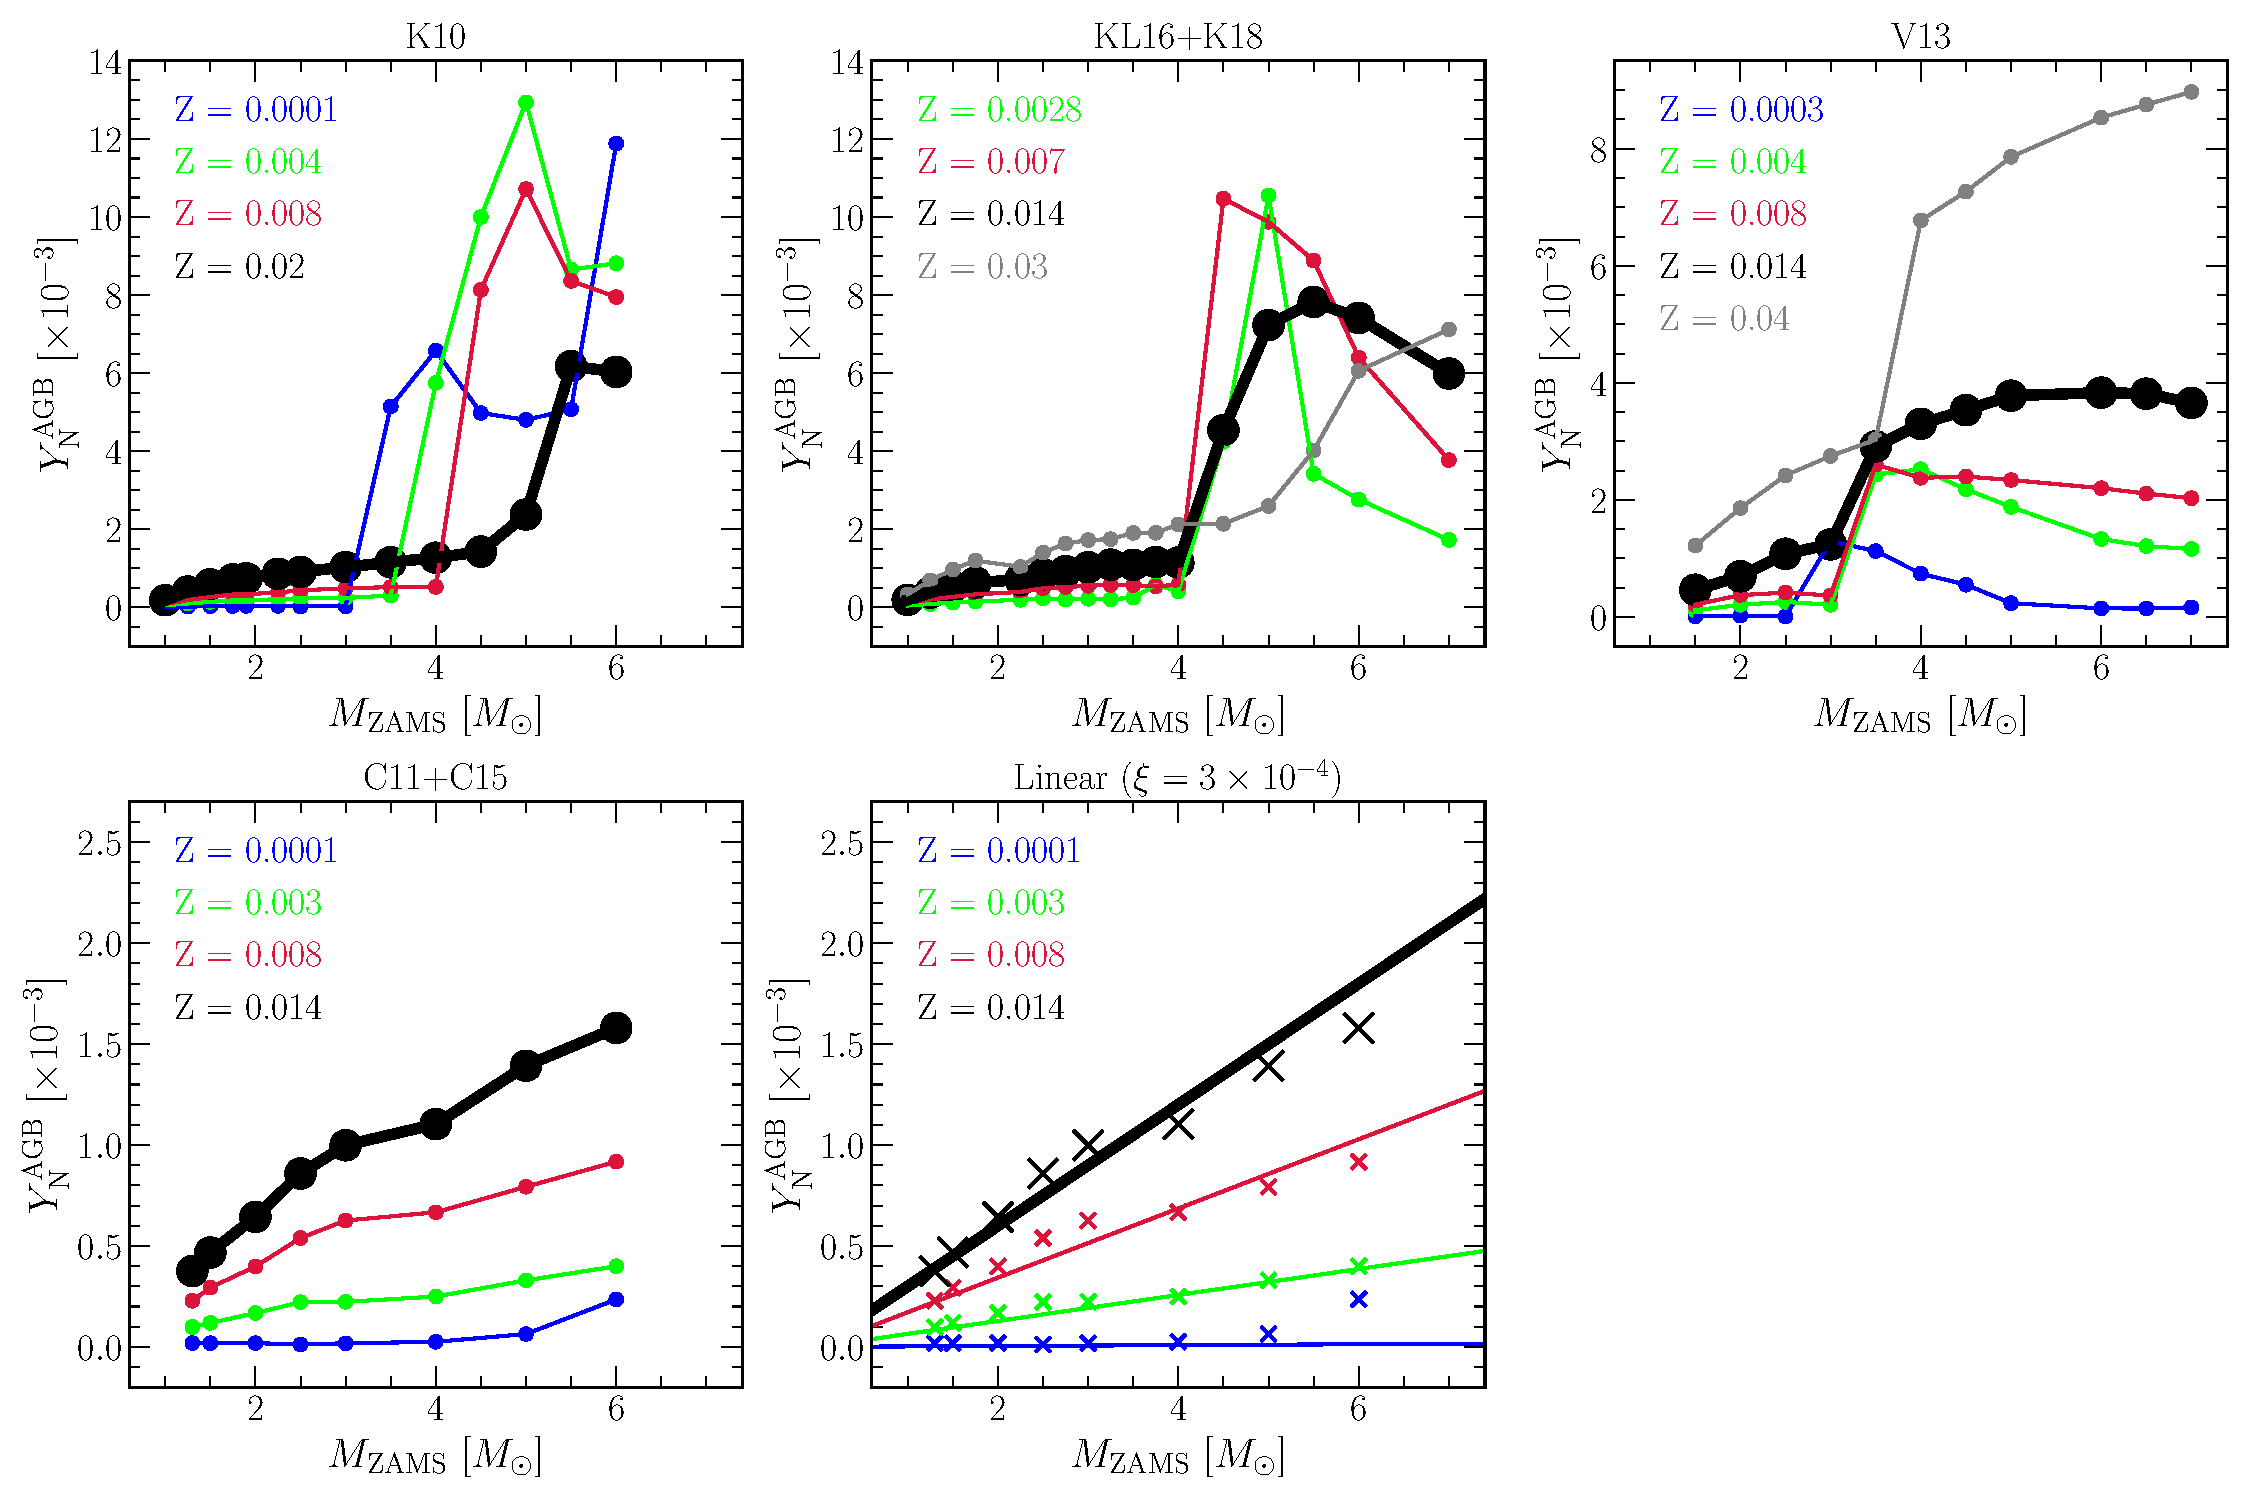
\includegraphics[scale = 0.45]{agb_yield_models.pdf}
\caption{
The fractional yields of N from AGB stars~\yagb{N}~as a function of progenitor
ZAMS mass and birth metallicity~$Z$ as reported by
\citet[][upper left]{Karakas2010},~\citet{Karakas2016} and
\citet[][upper middle]{Karakas2018},~\citet[][upper right]{Ventura2013,
Ventura2014, Ventura2018, Ventura2020}, and~\citet[][lower left]{Cristallo2011,
Cristallo2015}.
For~\citet{Ventura2013, Ventura2014, Ventura2018, Ventura2020} and
\citet{Cristallo2011, Cristallo2015}, we show the yields only for a selection
of metallicities available from their provided tables.
We highlight yields at solar metallicity ($Z = 0.02$ for~\citealp{Karakas2010},
$Z = 0.014$ otherwise) with bold black lines.
In the lower right panel, we show our linear model (coloured lines, see
equation~\ref{ohno:eq:linear_yield}) in comparison to
the~\citet[][coloured X's]{Cristallo2011, Cristallo2015} predictions.
We caution that the y-axis ranges are not the same between panels in this
figure.
}
\label{ohno:fig:agb_yield_models}
\end{figure*}

The~\citet{Sukhbold2016} tables, available only at solar metallicity, agree
nearly perfectly with our empirical value of~$\ycc{N} = 3.6\times10^{-4}$, but
they predict a higher value of~\no\subcc~by~$\sim$0.2 dex.
This is a consequence of the failed supernovae incorporated into their model
and the lowered values of~\ycc{O} that result (see discussion
in~\S~\ref{ohno:sec:results:yields}).
While N emerges in substantial amounts in winds, much of the O produced by
massive stars is ejected during the explosion, making the O yield more
sensitive to the black hole landscape~\citep{Griffith2021b}.
Most of the SN models plotted in Fig.~\ref{ohno:fig:n_cc_yields} estimate slightly
higher~\no\subcc~at~$\log_{10}(Z / Z_\odot)$ = 0 relative to our empirical
value of~\no\subcc~=~$-0.7$, but they still fall short of solar~\no.
This implies the need for an additional enrichment channel, which is expected
because it is well understood that N is also produced in considerable amounts
by AGB stars~\citep[e.g.][]{Johnson2019}.
% Although our empirically calibrated N yield agrees well with
% the~\citet{Limongi2018} predictions, massive star nucleosynthesis models
% overwhelmingly neglect the impact of a potential binary companion,
% and~\citet{Limongi2018} is no exception.
% \citet{Farmer2021} recently investigated the impact of binary star evolution on
% theoretically predicted yields and found a considerable increase in C
% production.
% Despite being an interesting possibility, GCE models with such yields are beyond
% the scope of this paper.

\subsection{Asymptotic Giant Branch Stars}
\label{ohno:sec:yields:agb}

% {\color{red}
% \sout{
% Similar to SNe, our AGB star yields are parametrized as fractional net yields.
% For a yield~$\yagb{X}$, the mass yield is given by~$M_\star \yagb{X}$.
% }
We use~\yagb{X} to denote the fractional net yield of an AGB star of mass
$M_\star$, so that the mass yield is~$M_\star\yagb{X}$.
We then define the IMF-averaged yield~$y_\text{X}^\text{AGB}$ by integrating
over the mass range~$M_\star = 1 - 8$~\msun.
% }
Enrichment proceeds as it does in~\citet{Johnson2021}: AGB stars place their
nucleosynthetic products in the~$\delta\rgal = 100$ pc ring that they are in at
a given time, allowing stars to enrich distributions of radii as they migrate.
\vice~implements an algorithm that computes the mass in dying stars
from each stellar population, and the zero age main sequence (ZAMS) mass
required to compute the fractional yield comes from a mass-lifetime
relationship. 
For the latter, we adopt the metallicity-independent parabola in
$\log\tau - \log m$ space from~\citet{Larson1974} with updated coefficients
from~\citet{Kobayashi2004} and~\citet*{David1990} (see discussion of the
mass-lifetime relationship in~\vice~in Appendix~\ref{ohno:sec:vice}).
\par
We make use of four previously published tables of AGB star N yields
computed from stellar evolution models, each of which are sampled on a grid
of progenitor masses and metallicities.
To approximate the net yield~\yagb{X}~as a smooth function of~$M_\star$ and
$Z_\star$,~\vice~interpolates bi-linearly -- once in mass~$M$ and once in
metallicity~$Z$ -- and linearly extrapolates above or below the grid in either
quantity as necessary.
By comparing the predicted abundances of the~\citet{Johnson2021} Milky Way
model to the latest observational data, we can constrain how accurately these
``off-the-shelf'' yield models characterize N production.
These models taken from the literature are as follows.
\begin{itemize}
	\item[\textbf{1.}] \citeauthor{Karakas2010} (\citeyear{Karakas2010};
	hereafter~\karakasten)\footnote{
		We clarify that our abbreviations of each of these papers refer
		specifically to their yields of N as we adopt them in our model.
		We cite the full names of these papers when referring to their more
		general results.
	} published yields for~$Z = 0.0001$, 0.004, 0.008, and 0.02 progenitors.
	We plot these yields in the upper left panel of 
	Fig.~\ref{ohno:fig:agb_yield_models}.

	\item[\textbf{2.}] \citet{Karakas2016} and~\citet{Karakas2018} published
	yields for~$Z = 0.0028$, 0.007, 0.014, and 0.03 progenitors; we hereafter
	refer to these yields as the~\karakas~model.
	We illustrate these yields in the upper middle panel of
	Fig.~\ref{ohno:fig:agb_yield_models}.

	\item[\textbf{3.}] We combine the yields for~$Z = 0.0003$ and 0.008
	progenitors from~\citet{Ventura2013} with those at~$Z = 0.004$ from
	\citet{Ventura2014}, at~$Z = 0.014$ from~\citet{Ventura2018}, and at
	$Z = 0.04$ from~\citet{Ventura2020} into a single table of yields.
	In this set, we also include a set of un-published yields at~$Z = 0.001$
	and 0.002 computed from similar models (provided by P. Ventura, private
	communication).
	We hereafter refer to this yield set as the~\ventura~model, and we plot a
	subsample of these yields in the upper right panel of
	Fig.~\ref{ohno:fig:agb_yield_models}.

	\item[\textbf{4.}] The default set of AGB star yields in~\vice~is taken
	from~\citet{Cristallo2011, Cristallo2015}, who published yields for
	$Z = 0.0001$, 0.0003, 0.001, 0.002, 0.003, 0.006, 0.008, 0.01, 0.014, and
	0.02 progenitors.
	We hereafter refer to these yields as the~\cristallo~model, and we
	illustrate a subsample of them in the lower left panel of
	Fig.~\ref{ohno:fig:agb_yield_models}.
\end{itemize}
\par
\vice~also allows users to construct their own functions of progenitor mass
and metallicity to describe the AGB star yield.
Motivated by the roughly linear nature of the~\cristallo~yields and their
general success once renormalized by a constant factor (see discussion
in~\S~\ref{ohno:sec:results:yields}), we construct a model in which the yield is
linearly proportional to both progenitor ZAMS mass and metallicity:
\begin{equation}
\yagb{N} = \xi \left(\frac{M_\star}{M_\odot}\right)
\left(\frac{Z_\star}{Z_\odot}\right).
\label{ohno:eq:linear_yield}
\end{equation}
We illustrate this model in the lower middle panel of Fig.
\ref{ohno:fig:agb_yield_models} for~$\xi = 3\times10^{-4}$ in comparison to
the~\cristallo~yields shown by the coloured X's.
Although we find good agreement between the~\cristallo~yields and our linear
model with a normalization of~$\xi = 3\times10^{-4}$, for our fiducial AGB star
yield of N we take a slope of~$\xi = 9\times10^{-4}$.
We discuss the absolute scaling of our nucleosynthetic yields
in~\S~\ref{ohno:sec:results:yields} below.
\par
As is clear from Fig.~\ref{ohno:fig:agb_yield_models}, the N yields reported by
these studies show substantial differences.
Unfortunately, ascertaining the origin of these differences is difficult
because each model employs its own assumptions for important evolutionary
parameters such as opacity, mass loss, nuclear reaction networks, and
convection and convective boundaries within stars, all of which have a
significant impact on stellar evolution and thus the predicted yields
% {\color{red}
% \sout{
% \mbox{\citep[see discussion in, e.g.,][]{Karakas2016}}.
% }
% }
% {\color{red}
\citep{Karakas2014, Karakas2016, Ventura2016, Ventura2018}.
% }
However, the differences can be qualitatively understood by considering two
important phenomena known to occur within AGB stars: TDU\footnote{
	The time adverbial ``third'' in TDU refers only to the fact that these
	dredge-up episodes are occurring while the star is on the asymptotic giant
	branch. Because they are associated with the thermal pulsations of AGB
	stars, there are many episodes of third dredge-up.
} and HBB.
The variations in how TDU and HBB proceed between different stellar evolution
models arise as consequences of the different input physics.
\par
When an AGB star experiences a thermal pulse,
% {\color{red} \sout{pulsation} pulse},
this is usually accompanied
by a TDU event whereby the convective envelope penetrates into the
hydrogen-depleted core, mixing some of this material with other material
exposed to partial He-shell burning.
The~\Cthirteen($\alpha$, n)\Osixteen~reaction, which is the main source of free
neutrons in low-mass AGB stars~\citep{Gallino1998}, can occur at substantial
rates when this core material is mixed with the He-rich shell.
This process does not directly affect N abundances in the shell because the
core is mostly composed of C and O at this evolutionary phase,
but~\Nfourteen~plays an important role in shaping an AGB star's overall
\textit{s}-process yield by acting as an efficient catalyst of neutron decay
via the~\Nfourteen(n, p)\Cfourteen($\beta^+~\nu_{e}$)\Nfourteen~reaction, the
first step of which is a resonant neutron capture~\citep{Cristallo2011}.
\par
HBB refers to proton capture reactions at the base of the convective envelope,
activating the CNO cycle and producing large amounts of~\Nfourteen~at the
expense of C and O isotopes
% {\color{red}
\citep*[e.g.,][]{Scalo1975, Bloecker1991}.
% \sout{
% HBB requires a higher mass AGB star progenitor ($M_\text{ZAMS} = 4 - 5~M_\odot$
% at~$Z_\odot$ according to~\mbox{\citealt{Karakas2010}}) than TDU
% ($M_\text{ZAMS} = 2 - 2.5~M_\odot$ at~$Z_\odot$ according to
% \mbox{\citealt{Karakas2010}}), but the minimum mass for both decreases at lower
% metallicities.
% }
HBB requires a minimum temperature slightly above~$10^7$ K at the base of the
convective envelope~\citep[e.g.,][]{Sackmann1991}, which in turn requires a
high mass AGB star progenitor.
For comparison, HBB occurs in the~\citet{Karakas2010} models for solar
metallicity stars at~$M_\text{ZAMS} = 4 - 5$~\msun~and up, whereas TDU occurs
at~$M_\text{ZAMS} = 2 - 2.5$~\msun and up.
The minimum mass for both decreases at lower metallicities because these stars
are both hotter and more compact.
% }
\par
The most efficient N production occurs when both TDU and HBB are active within
an AGB star, because each replenishment of C and O isotopes by TDU adds new
seed nuclei for the CNO cycle with HBB.
This is the reason for the substantial increase in yields at~$\sim$4~\msun~in
the~\karakasten~and~\karakas~models; in both yield sets, every star that
experiences HBB also experiences TDU (see, e.g., table 1
of~\citealp{Karakas2010}).
Their high mass AGB star yields are higher at low~$Z$ because both HBB and TDU
are more efficient~\citep[see discussion in][]{Ventura2013}: when the
metallicity is low, each TDU episode is deeper due to the lower opacity, and
the base of the convective envelope is hotter, increasing the rate of CNO cycle
reactions in HBB.
This interaction between TDU and HBB is also the reason for the increase in
the~\ventura~yields near~$\sim$3~\msun, but unlike
the~\karakasten~and~\karakas~models, their stars experience both processes only
in this narrow range of mass.
\par
Of all of these yields taken from the literature, the~\cristallo~sample shows
the smoothest dependence on progenitor mass and metallicity.
Below~$\sim$3~\msun, their agreement with the~\karakas~yields is good, but this
model has much lower N yields for higher mass AGB stars.
Pinpointing a single reason for this difference is difficult, even when
considering the differences between HBB and TDU.
Relative to the~\karakas~yields (see discussion in~\S~5 of
\citealp{Karakas2016}), the~\cristallo~stars have more mass loss, fewer
thermal pulses overall, and weaker HBB due to a lower temperature at the base
of the convective envelope. 
% {\color{red} \sout{each of which acts to lower the yield of~\Nfourteen.}
Each of these effects lower the yield of~\Nfourteen, but the latter is the
dominant one.
% }
\par
Although the~\karakasten~and~\karakas~yield models both show a substantial
increase in N yields above~$\sim$4~\msun, there are some noteworthy differences
between the two.
In the newer version, the yields at solar metallicity are somewhat higher,
and the yields at sub-solar metallicities decreased slightly, particularly for
the highest mass AGB stars.
These differences can be understood by slight variations in the input physics
(A. Karakas, private communication).
A portion of the increase in the yields at solar metallicity can be attributed
to the assumption of~$Z_\odot = 0.02$ versus~$Z_\odot = 0.014$\footnote{
	Changes in the accepted value of the metallicity of the sun trace back to
	the canonical value of~$\sim$2\% derived by, e.g.,~\citet{Anders1989} and
	\citet{Grevesse1998}, later being revised to~$\sim$1.4\% by, e.g.,
	\citet{Lodders2003} and~\citet*{Asplund2005}. See Table 4 of
	\citet{Asplund2009} for a compilation of measured values.
} and the impact this has on both HBB and TDU, but it does not account for the
entire difference.
% {\color{red}
% \sout{
% As a consequence of updates to opacity tables and the adopted solar composition,
% the~\karakas~models at solar metallicity are slightly hotter and more compact,
% giving them hotter HBB and deeper TDU.
% }
These stars are also slightly hotter and more compact due to updated opacity
tables, giving them hotter HBB and deeper TDU.
% }
With more thermal pulses overall and therefore a longer AGB lifetime, these
stars have more time to convert~\Ctwelve~into~\Nfourteen.
\karakas~also use low-temperature opacity tables based on~\citet{Marigo2002}
that follow the surface composition of the star more closely.
These opacities are high, making the
% {\color{red} \sout{more massive}
$Z = 0.007$
% }
AGB stars larger and increasing the mass-loss rate relative
to~\karakasten, truncating their N yields, 
% {\color{red}
particularly at the highest masses.
% }
The~$Z = 0.0028$ model uses the~\citet{Bloecker1995} mass-loss prescription
rather than that of~\citet{Vassiliadis1993}, which was used for
the~\karakasten~yields as well as the yields at other metallicities in
the~\karakas~model.
This choice results in fewer thermal pulses and a shorter AGB lifetime, giving
them less time to process C and O nuclei into~\Nfourteen.
\par
% {\color{red}
% \sout{
% In the interest of consistency, when we adopt a particular AGB star yield model
% for N, we also adopt the corresponding table within~\vice~for O and Fe when
% possible.}\footnote{
% 	\color{red}
% 	\sout{In the case of~\mbox{\citet{Ventura2013, Ventura2014, Ventura2018,
% 	Ventura2020}},
% 	AGB star yields of Fe are not available, and our linear model is only
% 	appropriate for N.
% 	In these cases, we assume the~\vice~default of the~\mbox{
% 	\citet{Cristallo2011, Cristallo2015}} yields for both O and Fe.}
% }
% \sout{These O and Fe yields, however,}
We do not discuss the AGB star yields of
O and Fe here as these quantities are negligible compared to their SN yields.
% }
Although we focus our investigation on AGB yields from~$\lesssim$~7~\msun~stars,
slightly more massive stars (up to~$\sim$12~\msun) sit near the critical mass
boundaries between different types of massive white dwarfs and electron capture
SN progenitors.
\citet{Doherty2017} investigated theoretically predicted yields of these stars
and found significant production of CNO isotopes.
There is also the intriguing possibility of the CNO yields from the earliest,
most metal-poor AGB stars (e.g. the~$Z = 10^{-5}$ models
of~\citealp{Gil-Pons2013, Gil-Pons2021}) and the insight this may afford into
N production at low~$Z$ and the most metal-poor stars in the Galaxy.
While experiments with such yields in our GCE models would be interesting, this
is beyond the scope of the current paper since our AGB yield models already
span a wide range of assumptions regarding stellar evolution.



\subsection{IMF-Averaged AGB Star Yields: Metallicity and Time Dependence}
\label{ohno:sec:yields:imf_agb}

% fig 4
\begin{figure*}
\centering
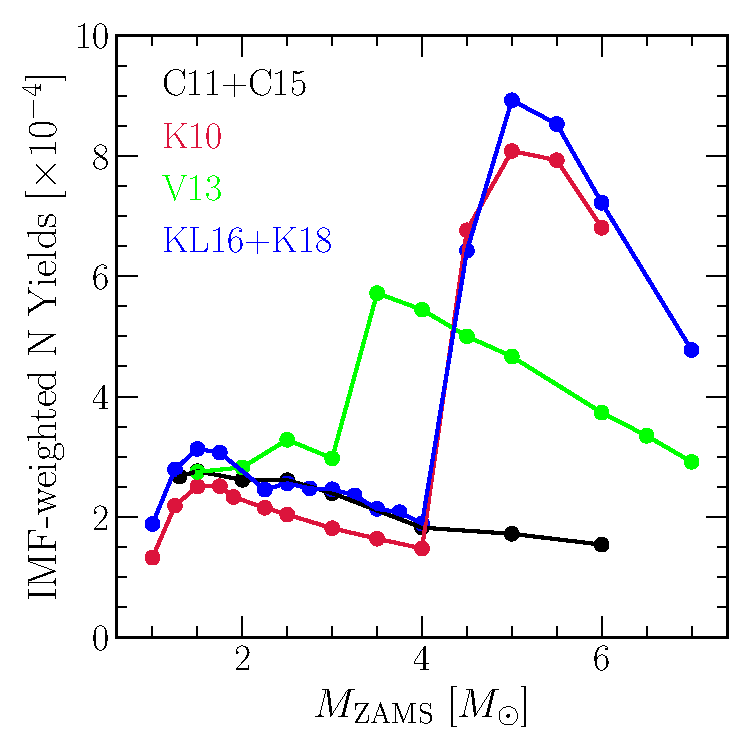
\includegraphics[scale = 0.46]{agb_yield_models_imfweighted.pdf}
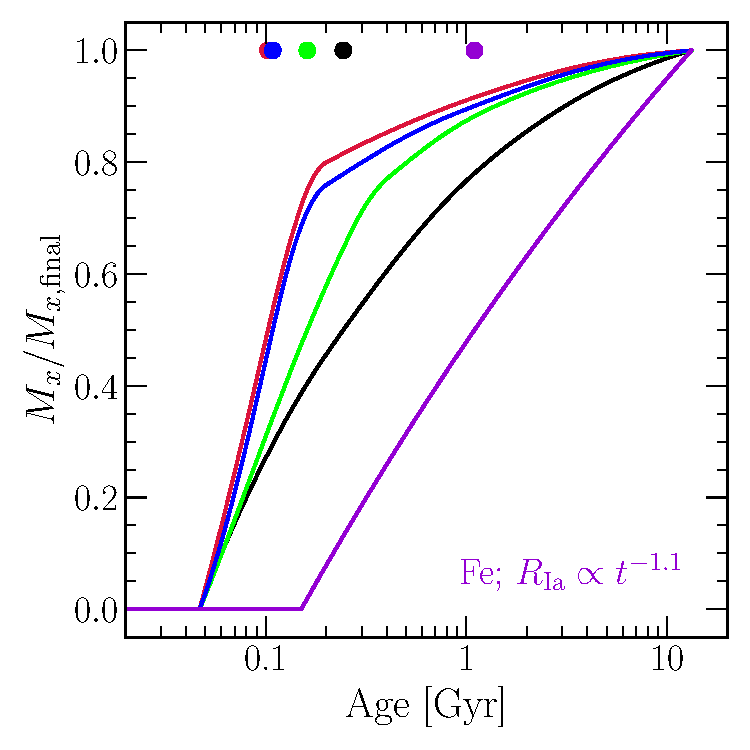
\includegraphics[scale = 0.45]{ssp_production_modelcomp.pdf}
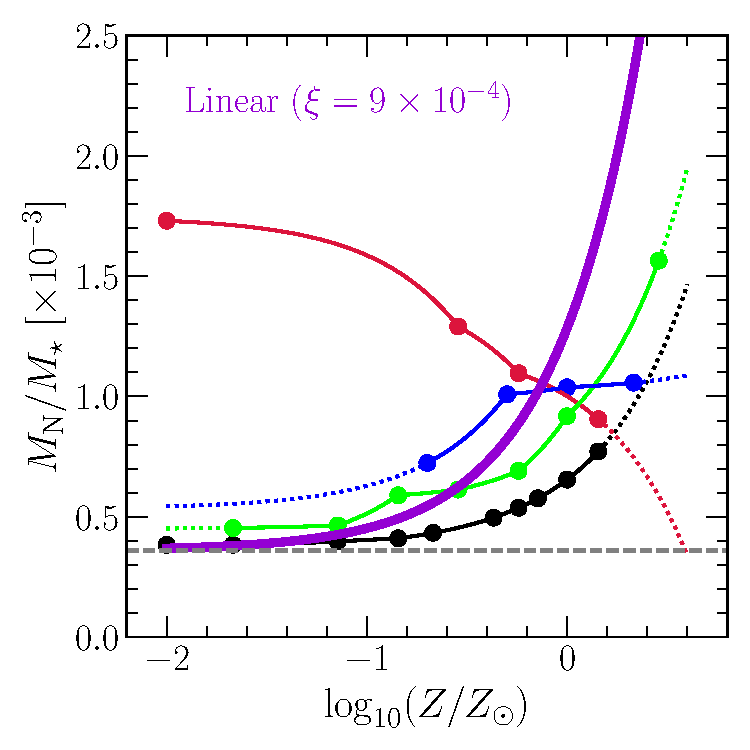
\includegraphics[scale = 0.46]{ssp_production_metdep.pdf}
\caption{
\textbf{Left}: The IMF-weighted mass yield of N from AGB stars as a function of
progenitor ZAMS mass at solar metallicity (i.e. the contribution per linear
interval~dM$_\text{ZAMS}$;~$Z_\odot = 0.014$).
\textbf{Middle}: The net mass of N produced by AGB stars from a single stellar
population for each of our yield models at solar metallicity.
The purple line denotes the same for Fe assuming our~$t^{-1.1}$ DTD as in the
\citet{Johnson2021} chemical evolution model.
All values are normalized to the total mass produced at an age of 13.2 Gyr.
Points at the top of the panel denote the ages at which 50\% of the total mass
yield has been produced.
\textbf{Right}: The total amount of N produced by a 13.2 Gyr old stellar
population as a function of metallicity for each of our yield models normalized
by the stellar population's initial mass.
Points mark metallicities at which the published tables report yields, and the
lines are dotted at metallicities that are above (below) the maximum (minimum)
metallicity reported by a given study (i.e. where extrapolation is necessary).
In this panel only, we include the metallicity-independent contribution
$\ycc{N} = 3.6\times10^{-4}$ from CCSNe (gray dashed line).
The bold purple curve represents our inference of the~\textit{total} N yield
(CCSN + AGB) required to reproduce the observational constrains discussed
in~\S~\ref{ohno:sec:results} given our adopted O and Fe yields (\S~\ref{ohno:sec:yields}).
}
\label{ohno:fig:ssp}
\end{figure*}

To more directly compare these AGB star yields predicted from stellar
evolution models, we plot their IMF-weighted yields at solar metallicity in the
left hand panel of Fig.~\ref{ohno:fig:ssp}.
We assume~$Z_\odot = 0.014$ based on~\citet{Asplund2009}
and~\citet*{Asplund2021}; since the~\karakasten~model reports yields at
$Z = 0.02$ rather than~$Z = 0.014$, we simply interpolate linearly
to~$Z = 0.014$ in the same manner that~\vice~does in our GCE models.
As mentioned in~\S~\ref{ohno:sec:yields:agb}, the AGB star yield~\yagb{N}~as we
have parametrized it is in units of the progenitor star's ZAMS mass, and
consequently the~\textit{mass yield} of N is given by~$M_\star \yagb{N}$.
With an additional weight of~$M_\star^{-2.3}$ from the IMF in this mass range
\citep[e.g.][]{Kroupa2001}, we therefore multiply the values of~\yagb{N}~by
$(M_\star / M_\odot)^{-1.3}$ to quantify a star's relative contribution to the
total N yield taking into account the intrinsic mass distribution.\footnote{
	This weight gives a contribution per linear interval of M$_\text{ZAMS}$, so
	one can use area under the curve to assess relative contributions.
}
With the additional weight of~$M_\star^{-1.3}$, the~\cristallo~yields are
relatively mass-independent.
For the other yield models, higher mass AGB stars dominate the overall yield
due to the effects of TDU and HBB discussed in~\S~\ref{ohno:sec:yields:agb}.
\par
Using~\vice's~\texttt{vice.single\_stellar\_population} function, in the
middle panel of Fig.~\ref{ohno:fig:ssp} we plot the total N yield as a function of
age from a single stellar population.
For the sake of this calculation, we set all CCSN yields of N to zero in order
to highlight the AGB star contribution.
We show the results of this procedure for solar metallicity only, and we
normalize all values
to the total mass produced at~$t = 13.2$ Gyr (the total amount of time our GCE
model is integrated over; see discussion in~\S~\ref{ohno:sec:multizone}).
Under the~\cristallo~yields, it takes~$\sim$250 Myr for a single stellar
population to produce~$\sim$50\% of its N from AGB stars, as noted by the
coloured points at the top of the panel.
This is in good agreement with~\citet{Maiolino2019}, who find that similar
parameter choices predict 80\% of the N yield to be ejected within~$\sim$1 Gyr
(see their fig. 1).
The characteristic timescales for N production are even shorter in the other
yield models because of their more pronounced contributions from massive stars
with short lifetimes~\citep[e.g.][]{Larson1974, Maeder1989, Padovani1993}.
For comparison, we plot the enrichment of Fe by our~$t^{-1.1}$ power-law DTD,
also with the CCSN yield set to zero to highlight the delayed component.
The characteristic delay time for Fe production is considerably longer than
that of N -- up to an order of magnitude depending on which yield model is
adopted.
As noted in~\citet{Johnson2021}, a characteristic delay time of~$\sim$1 Gyr
is exactly as expected for a~$\sim t^{-1}$ DTD because half of the SN Ia
events occur between 100 Myr and 1 Gyr and the other half between 1 Gyr and
10 Gyr.

% \begin{table}
% \caption{
% A summary of our AGB star yield models, where they are published/defined, and
% in which sections we present tests of each model.
% We take a fiducial value of~$\ycc{N} = 3.6\times10^{-4}$ for our IMF-averaged
% massive star yield (see discussion in~\S~\ref{ohno:sec:yields:ccsne}), and we
% explore alternate parametrizations of this value
% in~\S~\ref{ohno:sec:results:yields:yncc} only (right panel of
% Fig.~\ref{ohno:fig:no_oh_predictions}).
% }
% % \begin{tabularx}{\columnwidth}{l @{\extracolsep{\fill}} l r}
% \begin{tabularx}{\columnwidth}{p{2cm} @{\extracolsep{\fill}} p{3.2cm} r}
% \hline
% Model & Reference/Definition & Results
% \\
% \hline
% Linear & equation~\refp{ohno:eq:linear_yield} (fiducial yield) &
% % \ref{ohno:sec:results:fiducial} --~\ref{ohno:sec:results:schaefer_comp}
% % \ref{ohno:sec:results}.*
% \ref{ohno:sec:results:fiducial},~\ref{ohno:sec:results:yields:variations},
% \ref{ohno:sec:results:t_z_dep_comp},~\ref{ohno:sec:results:vincenzo_comp},
% \ref{ohno:sec:results:schaefer_comp}
% \\
% \cristallo & \citet{Cristallo2011, Cristallo2015} &
% \ref{ohno:sec:results:yields},~\ref{ohno:sec:results:yields:variations}
% \\
% \ventura & \citet{Ventura2013, Ventura2014, Ventura2018, Ventura2020} &
% \ref{ohno:sec:results:yields},~\ref{ohno:sec:results:yields:variations}
% \\
% \karakasten & \citet{Karakas2010} &
% \ref{ohno:sec:results:yields},~\ref{ohno:sec:results:yields:yncc}
% \\
% \karakas & \citet{Karakas2016, Karakas2018} &
% \ref{ohno:sec:results:yields},~\ref{ohno:sec:results:yields:yncc}
% \\
% \hline
% \end{tabularx}
% \label{ohno:tab:yields}
% \end{table}

A characteristic delay time of only~$\sim$250 Myr may seem surprising given
the relatively mass-independent nature of the IMF-weighted~\cristallo~yields.
This arises out of the steep nature of the stellar mass-lifetime relation
\citep[e.g.][]{Larson1974, Maeder1989, Padovani1993}.
For example, 2 and 3~\msun~stars live only~$\sim$1.2 Gyr and~$\sim$400 Myr,
respectively, and over the course of 13.2 Gyr, only stars of masses
$\gtrsim$0.9~\msun~will have enough time to finish their hydrogen burning.
Consequently, most of the mass range of stars that will evolve through an
AGB phase will do so within the first few hundred Myr after their formation,
and with mass-independent IMF-weighted yields, this accounts for most of the
N.
We clarify that the delay times computed here apply~\textit{only} to N and
not necessarily to other elements produced by AGB stars.
As we have illustrated here, the effective DTD of AGB star enrichment is
dictated by the combination of the stellar mass-lifetime relation and the
mass dependence of the yield, which should in principle differ from element to
element.
Other elements produced by slow neutron capture often have the highest yields
from lower mass AGB stars.
For example,~\citet{Cristallo2011, Cristallo2015} report Sr yields that are
dominated by~$M_\text{ZAMS} = 2 - 3~\msun$ progenitors (see fig. 5 of
\citealp{Johnson2020}), giving it a characteristic delay time of~$\sim$500 Myr.
The characteristic delay-times will be as long as a few Gyr if and only if the
yields are dominated by~$\lesssim$1.5~\msun~stars.
% We caution against interpretations of AGB star nucleosynthesis which attribute
% a single characteristic delay time to this enrichment channel as this is
% likely only accurate for order of magnitude estimates.
\par
In the right panel of Fig.~\ref{ohno:fig:ssp}, we plot the total amount of N
produced by a 13.2 Gyr old single stellar population as a function of its
initial metallicity according to all of our AGB star yield tables, including
the linear model (see equation~\ref{ohno:eq:linear_yield} and discussion
in~\S~\ref{ohno:sec:yields:agb}).
For this calculation, we include the metallicity-independent CCSN yield
($\ycc{N} = 3.6\times10^{-4}$; see discussion in~\S~\ref{ohno:sec:yields:ccsne}).
In general, there is good qualitative agreement between the~\cristallo~and
the~\ventura~models, the only major difference being the normalization.
The predictions with the linear model with~$\xi = 3\times10^{-4}$ are nearly
identical to the~\cristallo~model, as one would expect from
Fig.~\ref{ohno:fig:agb_yield_models}, but here we show the yields for our fiducial
choice of~$\xi = 9\times10^{-4}$.
The value at which these N yields flatten off at low~$Z$ is reflective of our
adopted value of~\ycc{N} (grey dashed line).
Up to~$\log_{10}(Z / Z_\odot) \approx -0.2$, the~\karakas~yields predict a
similar trend as~\cristallo~and~\ventura, also with a difference in
normalization, but at solar and super-solar metallicities they predict much
more metallicity-independent N yields than others.
The~\karakasten~yields, on the other hand, do not agree with any of the other
models, instead predicting N yields to~\textit{decrease} monotonically with
increasing~$Z$.
These differences between the~\karakasten~and~\karakas~models trace back to
differences regarding the opacity and mass loss prescriptions (see discussion
in~\S~\ref{ohno:sec:yields:agb}).
Although the normalization depends on the SN yields of all elements, we
demonstrate in~\S~\ref{ohno:sec:results:yields} that reproducing the~\ohno~relation
as observed requires AGB N yields which scale roughly linearly with metallicity
as in the~\cristallo~and~\ventura~models.
More specifically, with our adopted O and Fe yields (see discussion at the
beginning of~\S~\ref{ohno:sec:yields}), reproducing the observational constraints
that we consider requires~\textit{total} N yields (CCSN + AGB) with the
metallicity dependence shown by the purple curve in the right panel of
Fig.~\ref{ohno:fig:ssp}.

